\documentclass[11pt]{article}
\usepackage[utf8]{inputenc}
\usepackage[italian]{babel}
\usepackage{amssymb}
\usepackage{verbatim}
\usepackage{amsfonts}
\usepackage{amsmath}
\usepackage{multirow}
\usepackage{amsthm}
\usepackage{xcolor}
\usepackage{graphicx}
\usepackage{tikz}
\usepackage{float}
\usepackage[shortlabels]{enumitem}
\graphicspath{ {./images/} }
\usetikzlibrary{arrows}


\title{Titolo}
\author{Daniele De Micheli}
\date{2019}

\renewcommand*\contentsname{\textit{Indice}}

%presettaggio per teoremi e assiomi/definizioni%

\newtheorem*{nome}{teorema}

%fine%

\begin{document}

\maketitle
\tableofcontents

\part{Capitolo 1}
\section{Introduzione}
Questo documento è una sintesi degli appunti e dei concetti fondamentali necessari per poter affrontare con sicurezza l'esame di fisica nel nostro corso di studi. Come si può vedere dall'indice, il corso prevede tanti argomenti, che sono stati affrontati in modo non troppo approfondito e a volte forse in maniera superficiale. Spero di riuscire a creare una dispensa utile a chiunque voglia studiare senza dover comprare un libro e magari anche per chi per voglia o necessità non può seguire il corso fisicamente.
\subsection{Grandezze fondamentali e derivate}
Le \textit{grandezze fondamentali} e le \textit{grandezze derivate} sono \textbf{grandezze fisiche}, ossia caratteristiche di un corpo o di uno stato di un fenomeno che può essere misurata tramite strumenti ed esperimenti ed espressa tramite numeri e unità di misura.

Possiamo distinguere le due grandezze come segue:
\begin{itemize}
	\item Grandezze fondamentali: sono grandezze indipensdenti, cioè che non vengono definite a partire da altre grandezze. Alcuni esempi di grandezze fondamentali sono:
	\begin{itemize}
		\item Lunghezza: generalmente indicata con il simbolo L, è definita tramite il \textit{metro}, il quale è calcolato come la distanza che percorre la luce (nel vuoto), in un tempo di $\dfrac{1}{299729458}$ secondi.
		\item Tempo: si indica con la lettera T e rappresenta un concetto astratto. La sua unità di misura è il \textit{secondo} ed è calcolato come la durata di un determinato numero di oscillazioni complete di un atomo di Cesio 133.
		\item Massa: viene indicata dalla lettera M, la sua unità di misura è il \textit{chilogrammo} ed è definito tramite una proprietà fisica correlata ad una costante fondamentale, ossia come la quantità di massa per compensare una forza di $6,626 070 15 * 10^34$ J al s. 
		\item Temperatura: questa grandezza è rappresentata dalla lettera greca $\Theta$ e si misura in \textit{kelvin}.  Lo 0 kelvin è definito come \textit{zero assoluto}; il kelvin è inoltre definito come $\frac{1}{273,16}$ della temperatura del \textbf{punto triplo dell'acqua}.
	\end{itemize}
	\item Intensità di corrente: si indica con la lettera I, la sua unità di misura è l'\textit{ampere}. L'ampere è definito in maniera fisica come la forza di uno spostamento.
	\item Quantità di materia: viene indicata con la lettera N e si misura in \textit{mole}. Una mole corrisponde alla quantità di materia che contiene tante entità elementari quanti sono gli atomi presenti in 12 grammi di carbonio 12.
	\item Grandezze derivate: sono grandezze che nascono dalle grandezze fondamentali. Alcuni esempi di grandezze derivate che useremo sono:
	\begin{itemize}
		\item Volume: è una grandezza derivata definita come la misura nello spazio occupato da un solido.
		\item Velocità: è la quantità di spazio percorso rispetto ad una unità di tempo predefinita.
		\item Densità: rappresenta la quantità di massa in un'unità di volume.
	\end{itemize}
\end{itemize}

\subsection{Grandezze Scalari e Vettoriali}
Di grandezze ne esisitono di due tipi distinti, grandezze \textit{scalari} e grandezze \textit{vettoeiali}. Le prima sono rappresentabili tramite un semplice numero scalare, che rappresenta direttamente la "quantità" della grandezza. Per esempio, la temperatura è una grandezza scalare, come anche la massa.

Le grandezze vettoriali invece, possiedono delle caratteristiche oltre alla sola "quantità" di grandezza. Le proprietà sono 3:
\begin{itemize}
	\item \textbf{Modulo}: il modulo è la grandezza scalare della misura. Si potrebbe dire che è l'unica proprietà che possiedono le grandezze scalari.
	\item \textbf{Direzione}: rappresenta la direzione della grandezza. Di solito la direzione viene rappresentata tramite un segmento direzionato che giace su di una retta la quale indica la direzione del vettore.
	\item \textbf{Verso}: il verso rappresenta il "segno" della direzione; data un'origine è possibile capire rispetto ad essa se la grandezza è positiva o negativa.
\end{itemize}
Alcuni esempi di grandezze vettoriali sono la \textit{velocità} $\overrightarrow{v}$, l'accelerazione $\overrightarrow{a}$ o ancora la forza $\overrightarrow{F} = m*\overrightarrow{a}$, che è il prodotto di una grandezza scalare per una vettoriale.
\paragraph{Sistema di riferimento} Per poter utilizzare in modo corretto i vettori e le grandezze vettoriali, abbiamo bisogno di introdurre il concetto di \textit{\textbf{Sistema di riferimento}}: questo può essere visto come un'insieme di assi cartesiani che rappresentano lo spazio (monodimensionale, bidimensionale o tridimensionale). Generalmente utilizzeremo questi tre sistemi per rappresentare il mondo fisico che ci circonda.


Nello studiare un fenomeno, la scelta del sistema di riferimento è indipendente dallo spostamento.
\section{Cinematica}
\subsection{Velocità media e istantanea}
Prima di definire queste due grandezze, iniziamo con il definire i concetti di \color{red} distanza \color{black} e \color{red} spostamento\color{black}.
\\ \\
La \textit{distanza} è la quantità di spazio percorso in totale.
\\ \\
Lo \textit{spostamento} rappresenta, rispetto all'origine, di quando mi sono spostato. Potremmo vederla come una distanza relativa all'origine.

\begin{figure}[H]
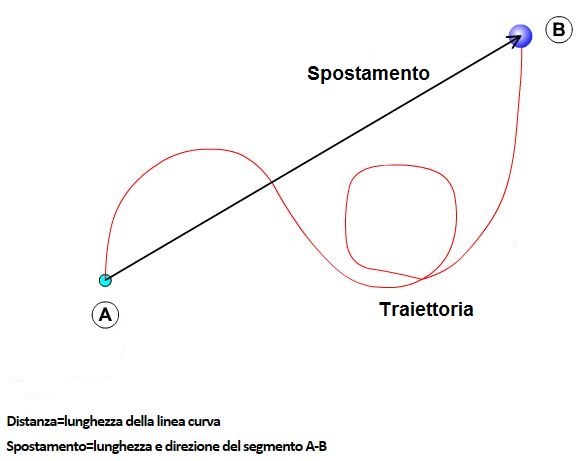
\includegraphics[scale=0.5]{distanza_spostamento.jpg}
\centering
\end{figure}

Un'altra convenzione che dobbiamo prendere riguarda il modo in cui consideriamo un oggetto. Nella nostra realtà, considereremo un oggetto come un \textit{punto  materiale}, dotato di massa.

\paragraph{Velocità media} Consideriamo uno spostamento $\Delta s$ e un intervallo di tempo $\Delta t$; definiamo la \textit{velocità media} come il rapporto tra lo spostamento e l'intervallo di tempo necessario affinché questo spostamento avvenga. In formula abbiamo che:
\begin{equation}
\label{EqVelocitàMedia}
v_m = \dfrac{spostamento}{intervallo \medspace di \medspace tempo} = \dfrac{\Delta s}{\Delta t}
\end{equation}

\subparagraph{Differenza tra velocità media e velocità media scalare} Consideriamo un viaggio di andata e ritorno in auto. La partenza è Milano, si arriva a Como e successivamente si torna a Milano.  Il tempo per il viaggio di andata (e poi di ritorno) è di 30 minuti, per un totale di 1 ora.

Se consideriamo la velocità media rispetto allo \textit{spostamento}, potremmo dire che $v_m = 0$, poiché lo spostamento totale risulta essere nullo. Difatti $v_m = \dfrac{0}{1} = 0 km/h$. Questo accade perchè come abbiamo già visto lo spostamento è la quantità di spazio percorsa rispetto all'origine (Milano). Partire da Milano e tornare a Milano implica uno spostamento nullo. 
\\ \\
Per quanto riguarda invece la velocità media rispetto alla \textit{distanza}, possiamo dire che si parla di \textit{velocità media scalare}. Difatti in questo caso, la distanza, rappresentata da uno scalare, rappresenta l'intero percorso tra Milano e Como e ancora Milano. Se l'andata Milano-Como è di 50 km, anche il ritorno è di 50 km e quindi in totale la distanza percorsa è di 100 km. In questo secondo caso possiamo allora dire che 
$$v_m = \dfrac{distanza}{intervallo di tempo} \dfrac{100}{1} = 100 \medspace km/h$$

In questo esempio abbiamo mostrato la differenza tra velocità media e velocità media scalare. Ora non ci resta che "sistemare" l'unità di misura. Infatti i km/h non sono l'unità di misura della velocità nel Sistema Internazionale. L'unità corretta è il "metro al secondo" (o m/s). La conversione tra una e l'altra è banale:

\begin{flalign*}
& \qquad \frac{km}{h} \rightarrow dividiamo \medspace per \medspace  3,6 \rightarrow \frac{m}{s} &&\\\nonumber
& \qquad \frac{m}{s} \rightarrow moltiplichiamo \medspace per \medspace  3,6 \rightarrow \frac{km}{h}&&\nonumber
\end{flalign*}


\paragraph{Velocità istantanea} La velocità istantanea è una grandezza \textit{vettoriale} definita come la derivata della posizione di un corpo rispetto al tempo.

Infatti, la velocità media non descrive in modo accurato il modo in cui un corpo si sta spostando: considerando sempre l'esempio di prima (Milano-Como-Milano), abbiamo calcolato la velocità media costante di 100 km/h, ma potrebbe benissimo essere che per i primi 15 minuti sono stato fermo, poi ho fatto 15 minuti a 200 km/h. La media risulta ancora 100 km/h, anche se di per se non è la stessa cosa che fare tutto il viaggio a 100 km/h.

Per descrivere meglio come si sposta un oggetto nello spazio rispetto al tempo utilizziamo infatti quella che abbiamo definito come \textit{velocità istantanea}. Prendiamo quindi un grafico spazio/tempo che rappresenta uno spostamento da un punto A ad un punto B.

\begin{figure}[H]
\label{veloIst1}
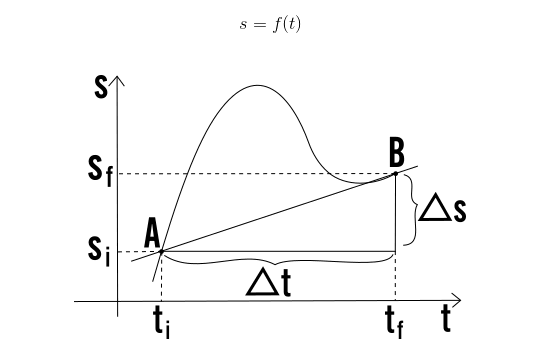
\includegraphics[scale=0.7]{velox_ist_1.png}
\centering
\end{figure}

Il tempo $\Delta t$ rappresenta la differenza tra il tempo finale e il tempo iniziale, mentre $\Delta s$ rappresenta lo spostamento. Con la rappresentazione soprastante però, non abbiamo una descrizione precisa: come possiamo vedere dal grafico, sappiamo che il corpo si muove molto velocemente all'inizio, per poi fermarsi, tornare indietro, fermarsi di nuovo e poi avviarsi lentamente verso il punto B.

La pendenza della retta che congiunge i due punti $A$ e $B$ (ovvero il suo coefficiente angolare) fornisce il valore della velocità media tenuta effettuando lo spostamento $\Delta s$ nel tempo $\Delta t$.
\begin{equation*}
m_{AB} = v_{m, AB} = \frac{\Delta s}{\Delta t}
\end{equation*}

Se a questo punto volessimo sapere in modo un po' più preciso come si sposta il corpo quando è vicino ad $A$, possiamo spostare $B$ più vicina ad essa. Prendiamo quindi un punto $B_1$ più vicino ad A tale che la sua velocità media risulta essere
\begin{equation*}
m_{AB'} = v_{m, AB'} = \frac{\Delta s'}{\Delta t'}
\end{equation*}

\begin{figure}[H]
\label{veloIst2}
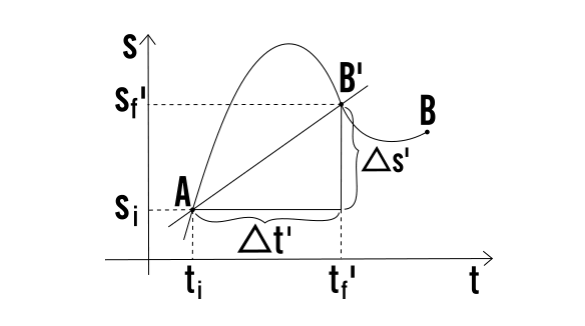
\includegraphics[scale=0.7]{velox_ist_2.png}
\centering
\end{figure}

Il nuovo valore di velocità è diverso da quello precedente, possiamo dire che rappresenta un intervallo minore e che quindi è un po' più preciso del precedente poiché descrive la velocità tra $A$ e $B'$. Possiamo notare anche che la pendenza della retta che passa per $A$ e $B'$ è più marcata.
Prendiamo ora un altro punto, $B''$, ancora più vicino ad $A$.
 \begin{figure}[H]
 \label{veloIst3}
 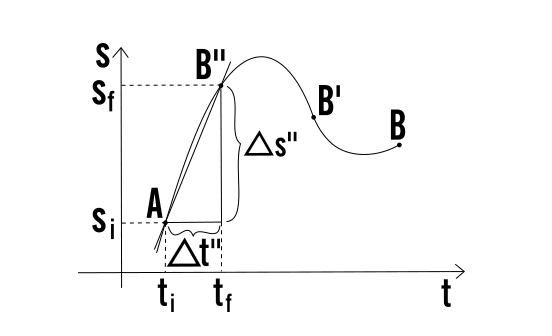
\includegraphics[scale=0.7]{velox_ist_3.png}
 \centering
 \end{figure}

Potremmo ricalcolare anche qui la velocità e sarebbe ancora diversa, ancora più precisa nei pressi di $A$. Il concetto alla base è proprio questo; ad ogni passo in cui ci avviciniamo ad $A$, l'intervallo di tempo si riduce sempre di più. 

Consideriamo allora un intervallo di tempo infinitesimale, \textit{prossimo allo zero}: vedremo che $B'''$ sarà in una posizione che quasi coincide con quella di $A$. Facendo questo notiamo che la retta che congiunge $A$ e $B'''$ non è più secante al grafico, ma diventa tangente ad esso. Quindi possiamo infine dedurre che la velocità istantanea non altro che la "pendenza" della tangente al grafico spazio-tempo in un punto.
\\ \\ 
Una definizione più formale di velocità istantanea è la seguente:
\begin{equation}
v = \lim_{\Delta t \to 0} \dfrac{\Delta s}{\Delta t} = \dfrac{ds}{dt}
\end{equation}
in cui $ds$ e $dt$ sono rispettivamente lo spostamento e l'intervallo di tempo infinitesimali, ovvero molto prossimi allo zero.

\subsection{Moto rettilineo uniforme}
Il\textit{ moto rettilineo uniforme} (o MRU) è il moto che descrive un corpo che si muove lungo una retta a velocità costante nel tempo. Tale moto è descritto dalla \textit{legge oraria del moto rettilineo uniforme}.

Passiamo subito ad un esempio pratico. Consideriamo un treno che viaggia da un punto $A$ a un punto $B$. Il moto del treno può essere descritto come quello di un punto materiale che si muove lungo una linea retta a velocità $\Delta \overrightarrow{v}$ costante.

\begin{figure}[H]
\label{motoRettilineoUniformeA-B}

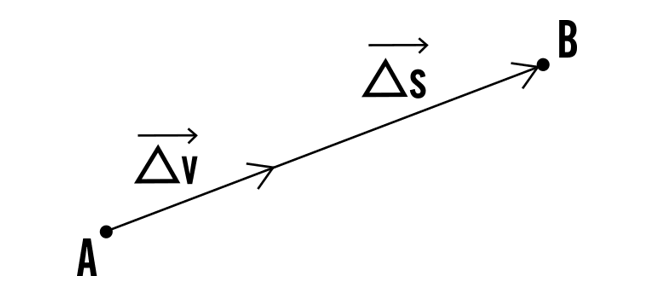
\includegraphics[scale=0.7]{moto_ret_unif.png}
\caption{Un moto rettilineo uniforme tra il punto A e il punto B}
\centering
\end{figure}

Per quanto riguarda questo tipo di moto, possiamo introdurre una tabella che riassume le formule del moto per poi presentare qualche esempio.



\section{Dinamica}
\section{Lavoro ed Energia}


Prendiamo un piano su cui poniamo una molla e un oggetto che si muove con velocità $v$ e con massa $m$.



\section{Gravitazione}
\part{Capitolo 2}
\section{Fluidodinamica}

\section{Termodinamica}

\section{Elettrostatica e Elettrotecnica}

\section{Magnetismo}




\end{document}
